\documentclass[12pt,a4paper]{article}

\usepackage{amsmath}
\usepackage{graphicx}
\usepackage{listings}
\usepackage{tcolorbox}
\usepackage{cancel}

\title{
	Understanding Linear Regression Through a Single Neuron\\
	{\large From Mathematical Foundations to Python Implementation}
}
\author{Michenchin}
\date{\today}

\definecolor{naranja}{HTML}{e34907}
\definecolor{rojo}{HTML}{d10202}

\newtcolorbox{NOTE}{
	colframe=naranja,
	title=\textbf{NOTE}
}

\newtcolorbox{WARNING}{
	colframe=rojo,
	title=\textbf{WARNING}
}

\begin{document}
	\maketitle
	\newpage
	% Aqui irá el indice que se irá creando a medida que voy poniendo
	% secciones, supongo.
	\tableofcontents
	\newpage
	
	% Empezamos con el documento de verdad
	\section{Before you begin}
		\begin{NOTE}
			You don't need to understand all the math explained in this document to grasp the basic concepts. Some people might even find it easier to read the code first and then come back to this document. I recommend having both the code and this document open
		\end{NOTE}
		\begin{WARNING}
			I'm not a teacher, mathematician nor expert in any of the topics covered in this project. I'm just an Spanish 17yo hobbyist trying to learn programming, AI, English, maths and LaTEX by myself that's why I did this project.
		\end{WARNING}
	% La introduccion
	\section{Introduction}
		\subsection{What is the project?}
			This project consists of a single-layer perceptron capable of performing linear regression given a dataset of X and Y points, the neuron automatically finds the best-fitting straight line that represents the trend of the data.\\
			\\
			To achieve this the neuron utilizes the Gradient Descent optimization algorithm. This method minimizes the prediction error in each iteration by adjusting the neuron internal weight and bias until the model achieves the most accurate linear relationship possible.\\
		\subsection{Project goals}
			This project goal is to understand and implement the math behind machine learning, using its simplest building block: a single neuron.
			The neuron will be trained to perform linear regression, and, ultimately, to accurately predict the values of $y$ for previously unseen values of $x$
	\section{Linear Regression}
		\subsection{What is linear regression?}
			linear regression is a model that estimates the relationship between a dependent variable and one or more explanatory variables independent variable.
		\subsection{The meaning of the variables}
			The neuron has two variables:
				\begin{enumerate}
					\item Weight: $w$
					\item Bias: $b$
				\end{enumerate}
			To do the prediction we will use:\\
			$$\hat{y_i}=wx_i+b$$
			So $w$ will be the slope of the line, and $b$ will be the y-intercept of the line
	\section{The Neuron}
		\subsection{How does it work?}
			The neuron receives an input, then passes it through a function and the output of the function is the prediction.
			\begin{figure}[h]
				\centering
				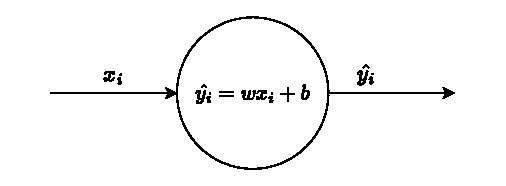
\includegraphics[width=0.5\textwidth]{../img/Single Neuron Schem}
				\caption{Schematic of how the neuron does a prediction}
				\label{single_neuron_schem}
			\end{figure}
		\subsection{Why a single neuron can perform linear regression}
			A single neuron can do linear regression because as seen in Fig.~\ref{single_neuron_schem} the intern structure of the neuron is exactly the equation of a straight line.
		\section{Measuring the error}
			\subsection{Loss Function}
				A Loss Function is a function we will use for measuring the error in the predictions, we will use the Mean Squared Error (MSE). The MSE is the squared sum of all the errors divided by de number of predictions. Our Loss Function will look like this:
				$$L(w,b) = \frac{1}{n} \sum_{0}^{n} (wx_i+b-y_i)^2$$
				The process is:
				$$(1)\	MSE=\sum_{0}^{n} (\hat{y_i}-y_i)^2$$
				$$(2)\	\hat{y_i}=wx_i+b$$
				And if we substitute $\hat{y_i}$ in the MSE function we get:
				$$L(w,b) = \frac{1}{n} \sum_{0}^{n} (wx_i+b-y_i)^2$$
				
		\section{The Gradient}
			\begin{WARNING}
				This part is the most mathematically complex, since it involves partial derivatives. Despite that, I'll try to explain it as clearly as possible.
			\end{WARNING}
			\subsection{Basic Concepts}
				\subsubsection{What is a derivative?}
					A derivative is a function in which you enter another function and the result is a new function which describes the exchange rate of the original function in each point.\\
					The mathematical definition of a derivative is this:
					$$f'(x) = \lim\limits_{h\to0}\frac{f(x+h)-f(x)}{h}$$
					An example with this definition and $x^2$
					$$f(x)=x^2$$
					$$f'(x) = \lim\limits_{h\to0}\frac{(x+h)^2-x^2}{h}$$
					If we expand the square binomial:
					$$f'(x) = \lim\limits_{h\to0}\frac{\cancel{x^2}2xh+h^2-\cancel{x^2}}{h}$$
					We factor out the common factor:
					$$f'(x) = \lim\limits_{h\to0}\frac{h(2x+h)}{h}$$
					We canceled the $h$:
					$$f'(x) = \lim\limits_{h\to0}\frac{\cancelto{1}{h}(2x+h)}{\cancelto{1}{h}}$$
					Now we have:
					$$f'(x) = \lim\limits_{h\to0}2x+h$$
					We apply the limit:
					$$f'(x) = 2x+0$$
					So:
					$$f'(x) = 2x$$
					This means that when in $f(x)\ x$ increases by one unit, its slope increases by 2.\\
					\\
					This is a standard derivative. We will use partial derivatives instead. The difference is that a standard derivative considers change in only one direction, whereas partial derivatives can consider changes in multiple directions. But the concepts are the same.
					\begin{NOTE}
						Standard derivatives are usually shown as $\frac{dy}{dx}$ and partial derivatives are shown as $\frac{\partial y}{\partial x}$
					\end{NOTE}
			\subsection{Derivative of the loss with respect to w}
				We need to find $\frac{\partial MSE}{\partial w}$\\
				We know that MSE depends on $\hat{y_i}$ and that $\hat{y_i}$ depends on $w$
				$$(1)\	MSE=\frac{1}{n}\sum_{0}^{n} (\hat{y_i}-y_i)^2$$
				$$(2)\	\hat{y_i}=wx_i+b$$
				So:
				$$MSE \longrightarrow \hat{y_i} \longrightarrow w$$
				Knowing this we can say that:
				$$\frac{\partial MSE}{\partial w} = \frac{\partial MSE}{\partial \hat{y_i}}\frac{\partial \hat{y_i}}{\partial w}$$
				\begin{NOTE}
					This is right not because the derivatives act as a fraction and can be canceled, but because of the chain rule. The total effect of changing $w$ is the effect of $w$ on $\hat{y}_i$, multiplied by the effect of $\hat{y}_i$ on the MSE.
				\end{NOTE}
				Now we have to find $\frac{\partial MSE}{\partial \hat{y_i}}$ and $\frac{\partial \hat{y_i}}{\partial w}$\\
				\\
				$$\hat{y_i}=wx_i+b$$
				$$\frac{\partial}{\partial w}\hat{y_i}=\frac{\partial}{\partial w}wx_i+b = x_i$$
				$$\boxed{\frac{\partial \hat{y_i}}{\partial w} = x_i}$$
				Because $b$ is a constant $\frac{\partial }{\partial w} b = 0$ and because We are differentiating with respect to $w$ $ \cancelto{1}{\frac{\partial }{\partial w}w}x_i = x_i$\\
				\\
				Now we are going to find  $\frac{\partial MSE}{\partial \hat{y_i}}$
				$$\frac{\partial}{\partial \hat{y_i}}MSE=\frac{\partial}{\partial \hat{y_i}}\sum_{0}^{n} (\hat{y_i}-y_i)^2$$
				$$\frac{\partial}{\partial \hat{y_i}}MSE=2\frac{1}{n}\sum_{0}^{n}(\hat{y_i}-y_i)$$
				$$\boxed{\frac{\partial MSE}{\partial \hat{y_i}} = \frac{2}{n}\sum_{0}^{n}(\hat{y_i}-y_i)}$$
				\\
				Now we can get $\frac{\partial MSE}{\partial w}$
				$$\frac{\partial MSE}{\partial w} = \frac{\partial MSE}{\partial \hat{y_i}}\frac{\partial \hat{y_i}}{\partial w}$$
				$$\boxed{\frac{\partial MSE}{\partial w} = \frac{2}{n}\sum_{0}^{n}(\hat{y_i}-y_i) x_i}$$
			\subsection{Derivative of the loss with respect to b}
				The process now is very similar as before.\\
				Now we need to find $\frac{\partial MSE}{\partial b}$\\
				We know that MSE depends on $\hat{y_i}$ and that $\hat{y_i}$ depends on $b$
				$$(1)\	MSE=\frac{1}{n}\sum_{0}^{n} (\hat{y_i}-y_i)^2$$
				$$(2)\	\hat{y_i}=wx_i+b$$
				So:
				$$MSE \longrightarrow \hat{y_i} \longrightarrow b$$
				Knowing this we can say that:
				$$\frac{\partial MSE}{\partial b} = \frac{\partial MSE}{\partial \hat{y_i}}\frac{\partial \hat{y_i}}{\partial b}$$
				Now we only have to find $\frac{\partial \hat{y_i}}{\partial b}$
				$$\hat{y_i} = wx_i+b$$
				$$\frac{\partial}{\partial b}\hat{y_i} = \frac{\partial}{\partial b}wx_i+b$$
				$$\boxed{\frac{\partial \hat{y_i}}{\partial b} = 1}$$
				Because $wx_i$ are constants $\frac{\partial }{\partial b} wx_i = 0$ and because we are differentiating with respect to $b$ $\cancelto{1}{\frac{\partial }{\partial b} b} = 1$\\
				\\
				Now we can get $\frac{\partial MSE}{\partial b}$
				$$\frac{\partial MSE}{\partial b} = \frac{\partial MSE}{\partial \hat{y_i}}\frac{\partial \hat{y_i}}{\partial b}$$
				$$\boxed{\frac{\partial MSE}{\partial b} = \frac{2}{n}\sum_{0}^{n}(\hat{y_i}-y_i)}$$
		\section{Gradient Descent}
			Now that we have $\frac{\partial MSE}{\partial w}$ and $\frac{\partial MSE}{\partial b}$ we will use that to adjust the predictions by adjusting the weight and bias.\\
			\\
			So after we do a prediction we adjust the weight and bias like this:
			$$w \leftarrow w - \eta \frac{\partial MSE}{\partial w}$$
			$$b \leftarrow b - \eta \frac{\partial MSE}{\partial b}$$
			Where $\eta$ is the learning rate.\\
			The \textbf{negative is important} because we want to move in the opposite direction of the gradient, towards a lower MSE.
				
				
				
		\section{Complete Cycle}
			\begin{enumerate}
				\item The neuron receives a list of points $x$
				\item Each point $x_i$ passes through the function $\hat{y_i} = wx_i+b$ and each point $\hat{y_i}$ is stored on the list of predictions
							\begin{figure}[h]
					\centering
					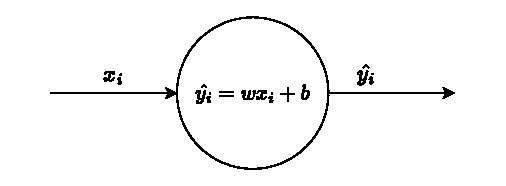
\includegraphics[width=0.5\textwidth]{../img/Single Neuron Schem}
				\end{figure}
				\item Given the prediction points $\hat{y}$ and the real points $y$ we calculate the MSE:
				$$MSE=\frac{1}{n}\sum_{0}^{n} (\hat{y_i}-y_i)^2$$
				\item Using the gradients $\frac{\partial MSE}{\partial w}$ and $\frac{\partial MSE}{\partial b}$ we adjust the weight and bias:
				$$w \leftarrow w - \eta \frac{\partial MSE}{\partial w}$$
				$$b \leftarrow b - \eta \frac{\partial MSE}{\partial b}$$
				\item Repeat until the error is as lowest as it can be.
			\end{enumerate}
			$$\boxed{x \longrightarrow \hat{y} \longrightarrow MSE \longrightarrow Gradients \longrightarrow w,\ b\ update \longrightarrow Repeat}$$

		\section{Personal Conclusion}
			This project helped me understand what is happening behind a simple neural network instead of just using it as a black box. I learned how predictions, loss functions, derivatives and Gradient Descent work together to make the neuron learn.
			
			This is only a small example, but it provides the mathematical foundations needed to understand more complex neural networks.
		\section{A final note}
			If you are reading this, I hope I explained everything clearly and that this document has helped you better understand how a neural network works.\\
			\\
			Thank you for reading! :)
		
\end{document}